\documentclass[12pt]{article}
\usepackage{alltt}
\usepackage[utf8]{inputenc}
\usepackage[dvips]{graphicx}
%\usepackage{a4wide}
\usepackage{epsfig}
\usepackage{fancybox}
\usepackage{verbatim}
\usepackage{array}
\usepackage{latexsym}
\usepackage{alltt}
%\usepackage{dsfont}
\usepackage{caption}
\usepackage{subcaption}
%\usepackage{fullpage}
\usepackage{hyperref}
\usepackage{textcomp}
\usepackage{listings}
\usepackage{color}
\usepackage{amsmath}
\usepackage{amsfonts}
\usepackage{tikz}
\usepackage{float}
\usepackage{matlab-prettifier}
\usepackage{graphicx}



\topmargin=-1.8cm
\addtolength{\textheight}{6.5cm}
\addtolength{\textwidth}{2.0cm}
\setlength{\oddsidemargin}{0.0cm}
\setlength{\evensidemargin}{0.0cm}

\newcommand{\HRule}{\rule{\linewidth}{1mm}}

\usepackage{tikz}
\usetikzlibrary{trees}
\tikzset{
  font={\fontsize{7pt}{12}\selectfont}}
  
\newcommand{\Q}{\raisebox{1.7pt}{$\scriptstyle\bigcirc$}}

\lstset{
    %backgroundcolor=\color{lbcolor},
    tabsize=2,
    language=C++,
    basicstyle=\footnotesize,
    numberstyle=\footnotesize,
    aboveskip={0.0\baselineskip},
    belowskip={0.0\baselineskip},
    columns=fixed,
    showstringspaces=false,
    breaklines=true,
    prebreak=\raisebox{0ex}[0ex][0ex]{\ensuremath{\hookleftarrow}},
    %frame=single,
    showtabs=false,
    showspaces=false,
    showstringspaces=false,
    identifierstyle=\ttfamily,
    keywordstyle=\color[rgb]{0,0,1},
    commentstyle=\color[rgb]{0.133,0.545,0.133},
    stringstyle=\color[rgb]{0.627,0.126,0.941},
}

\usepackage[]{mdframed}
\usepackage{enumitem}

\usepackage{titlesec}
\titleformat{\subsection}[runin]{}{}{}{}[]









\begin{document}

% Set the overall layout of the tree
\tikzstyle{level 1}=[level distance=2.5cm, sibling distance=20em]
\tikzstyle{level 2}=[level distance=2.5cm, sibling distance=10em]

% Define styles for bags and leafs
\tikzstyle{bag} = [text width=16em, text centered, align=center]
\tikzstyle{end} = [circle, minimum width=3pt,fill, inner sep=0pt]

\noindent
\HRule \\[3mm]
\small
\begin{tabular}[b]{lp{4.3cm}r}
Middle East Technical University &  &
Department of Computer Engineering \\
\end{tabular} \\
\begin{center}

                 \LARGE \textbf{CENG 280} \\[4mm]
                 \Large Formal Languages and Abstract Machines \\[4mm]
                \normalsize Spring 2022-2023 \\
                    \Large Homework 4 \\
\end{center}
\HRule



% Write down your name, surname, and student ID below.
\begin{center}
Name Surname:Doruk Berke Yurtsizoglu   \\
Student ID: 2522225
\end{center}



\section*{Answer for Q1}

\subsection*{1.} 
Context-free grammar that generates our language is:\\
\begin{center}

$S \rightarrow AX$\\
$A \rightarrow 0A0 | 1T1 | \#R$\\
$X \rightarrow XX | 0 | 1 | \epsilon$\\



\end{center} 

The PDA of this grammar:\\
K  = ($q_0$,$q_1$,$q_2$,$q_f$)\\
$\sum$ = (0,1)\\
$\gamma$ = (0,1,S,A,X)\\
F = (f)\\


I was not able to construct the rest of the PDA. Sorry about that :((((




\subsection*{2.}    

K = (s,$q_1$,$q_2$,f,$q_f$)\\
$\sum$ = (a,b,c)\\
$\gamma$ = (A,B,C)\\
F = (f)\\
$\Delta$:\\
1. ((s,c,e), (s,C))\\
2. ((s,e,e), ($q_1$,e)\\
3. (($q_1$,a,e), ($q_1$,A))\\
4. (($q_1$,b,e), ($q_1$,B))\\
5. (($q_1$,e,e), ($q_2$,e))\\
6. (($q_2$,a,A), ($q_2$,e))\\
7. (($q_2$,b,B), ($q_2$,e))\\
8. (($q_2$,e,e), (f,e))\\
9. ((f,c,C), (f,e))\\
10. ((f,e,e), ($q_f$,e)\\



\begin{center}
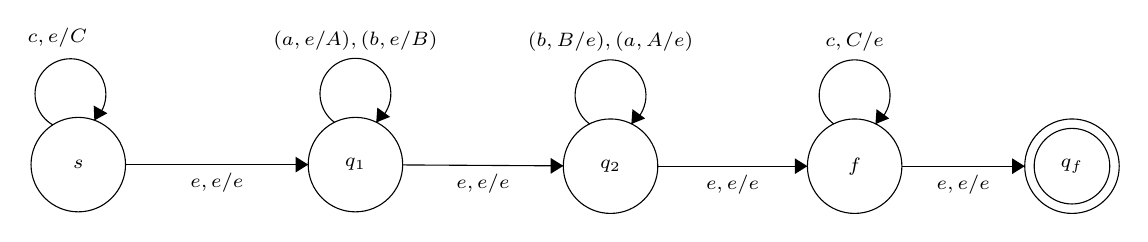
\begin{tikzpicture}[scale=0.2]
\tikzstyle{every node}+=[inner sep=0pt]
\draw [black] (11.5,-27.2) circle (3);
\draw (11.5,-27.2) node {$s$};
\draw [black] (29.1,-27.2) circle (3);
\draw (29.1,-27.2) node {$q_1$};
\draw [black] (45.3,-27.3) circle (3);
\draw (45.3,-27.3) node {$q_2$};
\draw [black] (60.8,-27.3) circle (3);
\draw (60.8,-27.3) node {$f$};
\draw [black] (74.6,-27.3) circle (3);
\draw (74.6,-27.3) node {$q_f$};
\draw [black] (74.6,-27.3) circle (2.4);
\draw [black] (9.89,-24.683) arc (240.34019:-47.65981:2.25);
\draw (10.17,-19.77) node [above] {$c,e/C$};
\fill [black] (12.52,-24.39) -- (13.35,-23.94) -- (12.48,-23.45);
\draw [black] (14.5,-27.2) -- (26.1,-27.2);
\fill [black] (26.1,-27.2) -- (25.3,-26.7) -- (25.3,-27.7);
\draw (20.3,-27.7) node [below] {$e,e/e$};
\draw [black] (27.777,-24.52) arc (234:-54:2.25);
\draw (29.1,-19.95) node [above] {$(a,e/A),(b,e/B)$};
\fill [black] (30.42,-24.52) -- (31.3,-24.17) -- (30.49,-23.58);
\draw [black] (32.1,-27.22) -- (42.3,-27.28);
\fill [black] (42.3,-27.28) -- (41.5,-26.78) -- (41.5,-27.78);
\draw (37.2,-27.76) node [below] {$e,e/e$};
\draw [black] (48.3,-27.3) -- (57.8,-27.3);
\fill [black] (57.8,-27.3) -- (57,-26.8) -- (57,-27.8);
\draw (53.05,-27.8) node [below] {$e,e/e$};
\draw [black] (63.8,-27.3) -- (71.6,-27.3);
\fill [black] (71.6,-27.3) -- (70.8,-26.8) -- (70.8,-27.8);
\draw (67.7,-27.8) node [below] {$e,e/e$};
\draw [black] (43.977,-24.62) arc (234:-54:2.25);
\draw (45.3,-20.05) node [above] {$(b,B/e),(a,A/e)$};
\fill [black] (46.62,-24.62) -- (47.5,-24.27) -- (46.69,-23.68);
\draw [black] (59.477,-24.62) arc (234:-54:2.25);
\draw (60.8,-20.05) node [above] {$c,C/e$};
\fill [black] (62.12,-24.62) -- (63,-24.27) -- (62.19,-23.68);
\end{tikzpicture}
\end{center}




\section*{Answer for Q2}

Counter Example: $(w \in (0,1)^* | $length of w is odd$)$ \\

G = (V, $\sum$, R,S), V = $(S) \cup \sum$, $\sum = (0,1)$\\

\begin{center}
		$S \rightarrow 0S0 | 0S1 | 1S0 | 1S1 | 0 | 1$
\end{center}
If we add the rule $S \rightarrow SS$ to the cfg that we defined, it will look like we get the kleene star of the language. However, kleene star of an expression includes the empty string which is not the case for our cfg since it doesn't have empty string in its rule set. That means we can't generate $L^*$ of the language we defined even if we add the rule $S\rightarrow SS$.\\

\section*{Answer for Q3}

\subsection*{1.} 

Just $L_1$.\\
\\
For $L_1$:(can be recognized as S-CFL)\\


		$\rightarrow$ Push all a's to the stack\\
		$\rightarrow$ When it is time to read b's, start to pop a's from the stack.\\
		$\rightarrow$ When the process is finished; if the stack is empty\\
		$\rightarrow$ Then the number of a's is equal to number of b's.\\


For $L_2$:(can't be recognized as S-CFL)\\

We can think of an algorithm which is similar to the language above, however it will not work because in the language $L_2$, the arrangement of a and b in the strings can be different. So we can't come up with an algorithm to recognize this language as a S-CFL.\\

For $L_3$:(can't be recognized as S-CFL)\\

		$\rightarrow$ Divide the strings to two parts.\\
		$\rightarrow$ $a^n b^n, b^m c^m$.\\
		$\rightarrow$ In order to check if the condition is satisfied, we need to have two symbols for stack symbols\\
		$\rightarrow$ Because we have to parts to compare.\\

\subsection*{2.} 

L = $(a^n b^m | n > m)$\\
G = (V,$\sum$,R,S)\\
V = (S, A, X) $\sum$
$\sum$ = (a,b)\\

\begin{center}
		$S \rightarrow Aa | XS | SXA$\\ 
		$A \rightarrow Aa | \epsilon$\\
		$X \rightarrow RR | aRb | bRa | \epsilon$\\
\end{center}

The process of PDA will be:\\

$\rightarrow$ Push all as' to the stack\\
$\rightarrow$ When it is time to read bs', start to pop as' from the stack.\\
$\rightarrow$ When the reading of bs' is finished;\\
$\rightarrow$ If there are still elements in the stack\\
$\rightarrow$ Then the number of as' is greater than number of bs'.\\

\subsection*{3.}  

One-Counter Automaton: A non-deterministic finite automaton with an addtional memory cell.\\

\subsection*{4.}  

The purpose of using an additional memory is to hold a non-negative integer. We are using this memory to copy the behavior of stack structure. Incrementing the integer is equal to adding something to the stack, decrementing the integer is equal to removing something fromthe stack, and checking if the integer is zero is equal to checking if the stack is empty.\\



\subsection*{5.}  

No, it is not closed under complementation. The reason for this is, the automons are non-deterministic. Let's look at the language $L_1$ from the part 1 of this question. The complement of $L_1$ is the string where the number of a is not equl to number of b. However the complement of $L_1$ still accepts the empty string which shouldn't be in the set of strings it accepts. So, we can say that, the class
of S-CFLs is not closed under complementation.\\




\end{document}
